\section{Materials and Methods}

\subsection{Materials}
%This research utilized several essential tools and libraries critical for data processing, analysis, and model evaluation within the ML framework. Python was chosen due to its versatility and robustness in handling data and ML tasks.
This research utilized several essential tools and libraries for data processing, analysis, and model evaluation within the ML framework.
A concise overview of the frameworks used is provided to the reader below, along with the motivation for their use according to their respective purposes:


\begin{itemize}
    \item \textbf{Numpy:} For efficient manipulation and mathematical operations on large datasets.
    \item \textbf{Pandas:} For reading, processing, and cleaning datasets, making them suitable for analysis and model training.
    \item \textbf{Matplotlib:} For creating visualizations to understand data distributions, relationships, and model performance.
    \item \textbf{Scikit-Learn (Sklearn):} For implementing and evaluating ML models, including tools for model selection, training, and validation.
\end{itemize}
%\textbf{Numpy:} \\
%Numpy is a foundational package for numerical computing in Python, providing support for large, multi-dimensional arrays and matrices, along with a collection of mathematical functions to operate on these arrays. It was used for efficient manipulation and mathematical operations on large datasets, enabling complex calculations with ease and precision.

%\textbf{Pandas:} \\
%Pandas is a powerful data manipulation and analysis library for Python, offering data structures like DataFrames ideal for handling and analyzing structured data. It facilitated the reading, processing, and cleaning of datasets, ensuring they were in a format suitable for analysis and model training. This library was crucial for transforming raw data into a usable form.

%\textbf{Matplotlib:} \\
%Matplotlib is a plotting library for Python and its numerical mathematics extension, Numpy. It provides an object-oriented API for embedding plots into applications. This library was employed to create various visualizations that helped understand data distributions, relationships, and the performance of ML models. Visual representation of data and results was key to interpreting the outcomes of the analysis.

%\textbf{Scikit-Learn (Sklearn):} \\
%Scikit-Learn is an open-source ML library for Python that features various classification, regression, and clustering algorithms, including support vector machines, random forests, GBM, k-means, and DBSCAN. It was used to implement and evaluate multiple ML models, offering tools for model selection, training, and validation, including metrics to assess model performance. This library provided a comprehensive suite of tools necessary for the development and evaluation of predictive models.


\subsection{Model Diagram}
The proposed procedure is comprehensively summarized in Figure-1 below, presented in the form of a model diagram. This figure systematically illustrates the sequential flow of the research conducted in constructing the predictive model for diabetes onset. Each stage of the process is represented to provide a clear and concise understanding of the methodology followed.

\begin{figure}[htpb!]
    \centering
    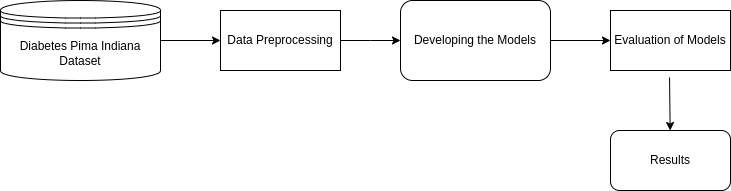
\includegraphics[width=0.5\textwidth]{Images/test.drawio.png}
    \caption{Flowchart of the Methodology for Predictive Model Construction}
    \label{fig:enter-label}
\end{figure}

\subsection{Data Preprocessing}

Data preprocessing is a crucial step in ML as it ensures that the dataset is clean, consistent, and suitable for analysis. Proper preprocessing helps in improving the model performance and making the analysis more reliable. For this study, the Pima Indian Diabetes dataset from Kaggle was used. This dataset includes features such as age, BMI, blood pressure, and glucose levels, which are essential indicators for predicting diabetes.

The preprocessing steps undertaken for this study were as follows:

\begin{enumerate}
    \item \textbf{Handling Missing Values}:
    \begin{itemize}
        \item The dataset had several instances where critical health metrics such as glucose, blood pressure, skin thickness, insulin, and BMI were recorded as zero, which is not possible in a real-world scenario. These zero values were treated as missing values.
        \item Missing values for glucose and blood pressure were replaced with the mean of the respective columns.
        \item For skin thickness, insulin, and BMI, the median values were used to replace the missing entries. Using the median is often more robust to outliers than the mean, especially in skewed distributions.
    \end{itemize}
    \item \textbf{Removing Outliers}:
    \begin{itemize}
        \item Outliers were identified through exploratory data analysis, including histograms and pair plots. However, explicit removal of outliers was not performed in this preprocessing step. Instead, normalization was employed to mitigate the impact of outliers on model training.
    \end{itemize}
    \item \textbf{Normalization}:
    \begin{itemize}
        \item Feature scaling was performed using the \texttt{StandardScaler} from \texttt{scikit-learn}, which standardizes the features by removing the mean and scaling to unit variance. This step ensures that all features contribute equally to the model training and helps in speeding up the convergence of gradient-based algorithms.
    \end{itemize}
    \item \textbf{Exploratory Data Analysis (EDA)}:
    \begin{itemize}
        \item EDA was conducted to understand the distribution of the data and the relationships between features.
        \item A pair plot was created to observe the pairwise relationships between features, colored by the outcome variable.
        \item A correlation heatmap was generated to identify the strength of relationships between features, helping in understanding multicollinearity which might affect model performance.
    \end{itemize}
    \item \textbf{Feature Selection}:
    \begin{itemize}
        \item Feature selection involves identifying the most relevant features that contribute to the prediction of diabetes. In this study, techniques such as correlation analysis and recursive feature elimination were employed to select the most significant features. The selected features were then used to train the ML models.
    \end{itemize}
\end{enumerate}

By performing these preprocessing steps, the dataset was transformed into a form that is optimal for training a ML model. This ensures that the models built on this data are robust, reliable, and capable of providing meaningful insights into the factors influencing diabetes.
An example heatmap generated for this dataset using a DT algorithm is shown in Figure~\ref{fig:correlation_heatmap}.
\begin{figure}[htpb!]
    \centering
    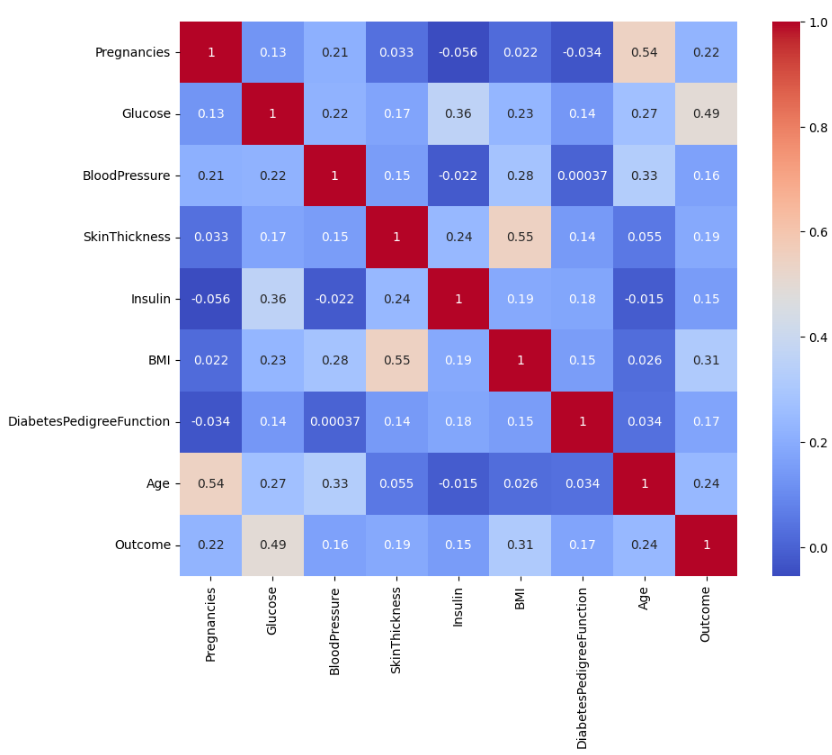
\includegraphics[width=0.4\textwidth]{Images/heatmap.png}
    \caption{Correlation heatmap of features in the Pima Indian Diabetes dataset.}
    \label{fig:correlation_heatmap}
\end{figure}

%Data preprocessing is a crucial step in ML as it ensures that the dataset is clean and suitable for analysis. This involves handling missing values, outliers, and normalizing the data. For this study, the Pima Indian Diabetes dataset from Kaggle was used. The dataset includes features such as age, BMI, blood pressure, and glucose levels. The preprocessing steps included handling missing values, removing outliers, and normalizing the data to ensure that all features contribute equally to the model training.


\subsection{Models Development}

The selected features were used to develop predictive models using various ML algorithms. These models were trained and validated to ensure their accuracy and robustness. The feature selection process, which included techniques such as correlation analysis and recursive feature elimination, ensured that only the most relevant features were used in model development. This process helps in reducing overfitting and improving the generalizability of the models.
To effectively predict diabetes onset, it is essential to leverage various ML algorithms, each with unique strengths and capabilities. The following advanced ML algorithms were implemented, each chosen based on its ability to handle different aspects of the dataset and the specific requirements of the prediction task:

\begin{itemize}
    \item \textbf{LR:} LR was used as a baseline model due to its simplicity and interpretability. It is a statistical method for analyzing a dataset where there are one or more independent variables that determine an outcome, predicting the probability of a binary outcome.
    \item \textbf{DT:} DTs were implemented to capture non-linear relationships in the data. This method splits data into subsets based on feature values, providing a visual interpretation of feature importance and decision rules.
    \item \textbf{RF:} RF, an ensemble method combining multiple decision trees, was utilized for its robustness in handling non-linear relationships and reducing overfitting. It aggregates the predictions of multiple trees to improve accuracy \cite{Ref11}.
    \item \textbf{SVM:} A model that finds the optimal hyperplane to separate different classes. SVMs are particularly useful for high-dimensional spaces.
    \item \textbf{GBM:} GBM builds models sequentially to correct errors from previous models, enhancing performance by focusing on difficult-to-predict cases. This iterative approach helps in achieving high predictive accuracy \cite{Ref12}.
    \item \textbf{XGBoost:} An advanced implementation of gradient boosting, was chosen for its efficiency and scalability. It leverages regularization to prevent overfitting and was one of the top-performing algorithms in this study \cite{Ref13}.
\end{itemize}

\subsection{Model Evaluation and Evaluation Metrics}

Model performance was evaluated using several key metrics to ensure comprehensive assessment and robustness. The primary metrics included:

\begin{itemize}
    \item \textbf{Accuracy}: Measures the proportion of correctly predicted instances among the total instances. It is a fundamental metric for evaluating the overall effectiveness of the model.
    \item \textbf{Precision}: The ratio of true positive predictions to the total predicted positives. Precision indicates the accuracy of positive predictions, essential for assessing the model's performance in identifying true cases of diabetes.
    \item \textbf{Recall (Sensitivity)}: The ratio of true positive predictions to the total actual positives. Recall measures the model’s ability to identify all actual positive cases, critical for ensuring no true cases of diabetes are missed.
    \item \textbf{AUC-ROC (Area Under the Receiver Operating Characteristic Curve)}: Represents the model's ability to distinguish between classes. A higher AUC-ROC value indicates better model performance in terms of distinguishing between diabetic and non-diabetic instances \cite{Ref14}.
\end{itemize}

These metrics were chosen for their ability to provide a multi-faceted view of model performance. Accuracy offers a general overview, while precision and recall provide deeper insights into the model's performance in correctly identifying positive cases and minimizing false negatives. The AUC-ROC metric complements these by offering an aggregate measure of performance across various thresholds, which is particularly useful for evaluating the trade-offs between sensitivity and specificity.

By employing these metrics, the evaluation ensures that the model not only performs well on a broad scale but also excels in the critical task of accurately identifying diabetic cases, thereby balancing the need for sensitivity and specificity in medical diagnostics. This comprehensive evaluation guides the selection and fine-tuning of models to achieve optimal performance in predicting diabetes.

